\section{Metodologia}\label{sec:metodologia}

Esta seção reúne os modelos físicos que definem o simulador estocástico, a formulação da função de estado limite dependente do tempo, o procedimento de construção do emulador (incluindo a camada temporal de aprendizado de máquina) e a ponte entre a distribuição emulada e as grandezas de gestão de ativos (probabilidade de falha, tempo até a falha, RUL e métricas de risco).

% =====================================================================
% 4.1 SIMULADOR ESTOCASTICO: DEFINICAO DO PROBLEMA
% =====================================================================
\subsection{Simulador estoc\'astico}
\label{subsec:carbonatacao}

A fundamentação sobre o mecanismo de degradação e o modelo de previsão da profundidade carbonatada foi apresentada na Seção~\ref{sec:vida_util}. Esta subseção define como esse modelo é organizado em um simulador estocástico: qual é a função de estado limite, como as variáveis são separadas entre entradas controladas e fontes latentes de aleatoriedade, e quais parametrizações foram adotadas.

\subsubsection{Fun\c{c}\~ao de estado limite de despassiva\c{c}\~ao}
\label{subsec:funcao_g}

Conforme estabelecido na Seção~\ref{subsec:degradacao}, o estado limite adotado é a despassivação da armadura, atingida quando a frente carbonatada alcança o nível do aço. A margem de segurança no instante $t$ é, portanto, a distância remanescente entre a face da armadura e a frente de carbonatação:

\begin{equation}\label{eq:funcao_g}
g(\mathbf{X}, t) = c(\mathbf{X}) - y(\mathbf{X}, t),
\end{equation}

\noindent em que $c$ é o cobrimento efetivo da armadura (mm) e $y$ é a profundidade de carbonatação (mm) dada pela Equação~\eqref{eq:y}. A interpretação física é direta:

\begin{equation}\label{eq:dominio_falha}
\begin{cases}
g(\mathbf{X}, t) > 0,    & \text{armadura passivada (per\'iodo de inicia\c{c}\~ao)}, \\[4pt]
g(\mathbf{X}, t) \leq 0, & \text{despassiva\c{c}\~ao (fim do per\'iodo de inicia\c{c}\~ao)}.
\end{cases}
\end{equation}

Trata-se de um estado limite de serviço de durabilidade: sua violação não corresponde à ruína da peça, mas ao encerramento da fase protegida e ao início da janela em que a corrosão pode se desenvolver. Consequentemente, as distribuições de vida útil remanescente obtidas neste trabalho, no sentido das Equações~\eqref{eq:ttf} e \eqref{eq:rul}, referem-se ao tempo até a despassivação.

\paragraph{Vari\'aveis de projeto e vari\'aveis latentes.} A estrutura da Equação~\eqref{eq:funcao_g} admite a separação exigida por um simulador estocástico (Seção~\ref{subsec:simulador}). O vetor $\mathbf{X} = \{f_c,\, UR,\, c_{\mathrm{nom}}\}$ reúne as \textit{variáveis de projeto}, que caracterizam a peça e o ambiente e distinguem um elemento de outro. Sobre elas atua um conjunto de \textit{variáveis latentes} $\boldsymbol{\omega}$, multiplicativas, que representam a dispersão interna ao próprio elemento --- heterogeneidade do material ao longo da peça, variabilidade executiva do posicionamento da armadura, flutuação das condições ambientais e erro do modelo de carbonatação:

\begin{equation}\label{eq:latentes}
f_c^{\,\ast} = f_c\,\omega_{f_c}, \qquad UR^{\ast} = UR\,\omega_{UR}, \qquad c = c_{\mathrm{nom}}\,\omega_{c}.
\end{equation}

Essa separação é o que confere ao problema a estrutura de simulador estocástico: para um mesmo vetor de projeto $\mathbf{x}$ e um mesmo instante $t$, a resposta $g$ não é um valor único, mas uma \textit{variável aleatória} cuja distribuição condicional precisa ser caracterizada. É precisamente essa distribuição condicional que o emulador da Seção~\ref{subsec:construcao_emulador} aproxima. \falta{fixar e justificar os coeficientes de varia\c{c}\~ao de $\omega_{f_c}$, $\omega_{UR}$ e $\omega_c$ com base em refer\^encias de variabilidade executiva (cobrimento) e no erro de modelo da Equa\c{c}\~ao~\eqref{eq:y}; declarar em Limita\c{c}\~oes que a correla\c{c}\~ao espacial ao longo da pe\c{c}a n\~ao \'e representada}

Determinada a trajetória de $g$ para cada realização, a repetição do procedimento para todos os instantes e todas as amostras permitiria, em princípio, obter as curvas de confiabilidade e a distribuição do tempo até a despassivação por simulação direta de Monte Carlo. O custo dessa estratégia quando se deseja varrer projetos, cenários de exposição e instantes de inspeção é justamente o que motiva o emulador proposto.

\subsubsection{Parametriza\c{c}\~ao adotada}
\label{subsec:parametrizacao}

Neste estudo adotou-se cimento CP~II~F e ambiente externo protegido da chuva ($k_{ce} = 1{,}00$), o que fixa os coeficientes $k_c = 21{,}68$, $k_{fc} = 1{,}50$, $k_{ad} = 0{,}24$, $k_{CO_2} = 18{,}00$, $k_{UR} = 1100$ e $k_{ce} = 1{,}00$ da Tabela~\ref{tab:coef_possan}. O teor de adição foi mantido em $ad = 10\%$. \falta{justificar o valor de $ad$ de forma independente --- teor t\'ipico de adi\c{c}\~ao para o cimento adotado, ou refer\^encia de pr\'atica brasileira --- e decidir se ele permanece fixo ou entra como vari\'avel do problema; note que $ad = 0$ reduz a profundidade carbonatada em torno de 1,6~mm nas condi\c{c}\~oes analisadas} Registra-se que, no modelo original, $ad$ refere-se a adições pozolânicas em relação à massa de cimento, ao passo que o CP~II~F é um cimento com fíler calcário; a interpretação desse parâmetro para o cimento adotado deve, portanto, ser explicitada.

Por fim, ressalta-se que a Equação~\eqref{eq:y} é avaliada neste trabalho em sua forma fechada, e não por meio de um metamodelo de aprendizado de máquina ajustado a ela. Essa opção garante que o emulador estocástico proposto na Seção~\ref{subsec:construcao_emulador} seja construído e validado contra o próprio modelo mecanístico de referência, sem a interposição de uma aproximação intermediária.

\subsubsection{Trajet\'oria de \texorpdfstring{CO$_2$}{CO2} e idade da estrutura}
\label{subsec:co2}

As trajetórias de concentração atmosférica adotadas foram apresentadas na Seção~\ref{subsec:co2_cenarios}. Descreve-se aqui como elas são associadas à idade da estrutura e convertidas na entrada do modelo de carbonatação.

Para associar a exposição ambiental à idade da estrutura, distingue-se o ano-calendário $a$ do tempo de exposição $t$:
\begin{equation}
    a = a_0 + t, \qquad 0 \leq t \leq T, \qquad a_0+T \leq 2100,
    \label{eq:co2_calendar_age}
\end{equation}
em que $a_0$ é o ano de início da exposição, tomado como o ano de construção, e $T$ é o horizonte de análise. Dessa forma, 100 anos correspondem a 1980--2080 para uma construção de 1980 e a 2000--2100 para uma construção de 2000. O horizonte de análise não é uma vida útil previamente assegurada; o atendimento ao critério de desempenho é avaliado ao longo desse intervalo.

Denotando por $C_s(a)$ a concentração em ppm para o cenário $s$, a entrada utilizada na Equação~\eqref{eq:y}, expressa em porcentagem, é
\begin{equation}
    CO_{2,s}(t)\,[\%] = \frac{C_s(a_0+t)}{10^4}.
    \label{eq:co2_conversion}
\end{equation}
Para anos inteiros, empregam-se diretamente os valores tabulados; para anos fracionários, realiza-se interpolação linear entre os dois anos adjacentes. Não se admite extrapolação fora de 1900--2100. O limite de disponibilidade da série ambiental não amplia o domínio de validade do modelo de carbonatação.

Adota-se a média global como uma hipótese de concentração atmosférica de fundo. Não são representadas diferenças locais associadas a tráfego, ventilação ou ocupação. Além disso, variar apenas o CO$_2$, mantendo as demais hipóteses ambientais, caracteriza uma análise de sensibilidade à concentração atmosférica, e não uma simulação conjunta de todos os efeitos das mudanças climáticas. As incertezas dos materiais e da exposição consideradas no simulador são avaliadas condicionalmente a cada trajetória de CO$_2$; a dispersão entre cenários não é tratada como intervalo probabilístico.

\paragraph{Perfis paramétricos de referência.} As Figuras~\ref{fig:evolution_fck} e \ref{fig:evolution_h} ilustram a resposta da Equação~\eqref{eq:y} para uma estrutura construída em 2000 e analisada até 2100, sob SSP2-4.5, cimento CP~II~F, exposição externa protegida e $ad=10\%$. Na primeira figura varia-se $f_c$ com $UR=65\%$; na segunda varia-se $UR$ com $f_c=30$~MPa. A linha em 30~mm corresponde ao cobrimento escolhido para essa ilustração, sem pretensão de representar todas as classes de exposição.

Nesses perfis, a expressão de carbonatação é avaliada com a idade e a concentração correspondentes a cada ano, aplicando-se o máximo acumulado para impedir a redução da profundidade. Essa é uma aproximação temporal da aplicação do modelo, não uma integração explícita do histórico de difusão e reação. A interpretação dos resultados está sujeita a essa limitação; a adoção de cenários publicados de CO$_2$ não constitui, por si só, validação dessa aproximação.

\begin{figure}[htbp]
    \centering
    \begin{subfigure}[b]{0.48\textwidth}
        \centering
        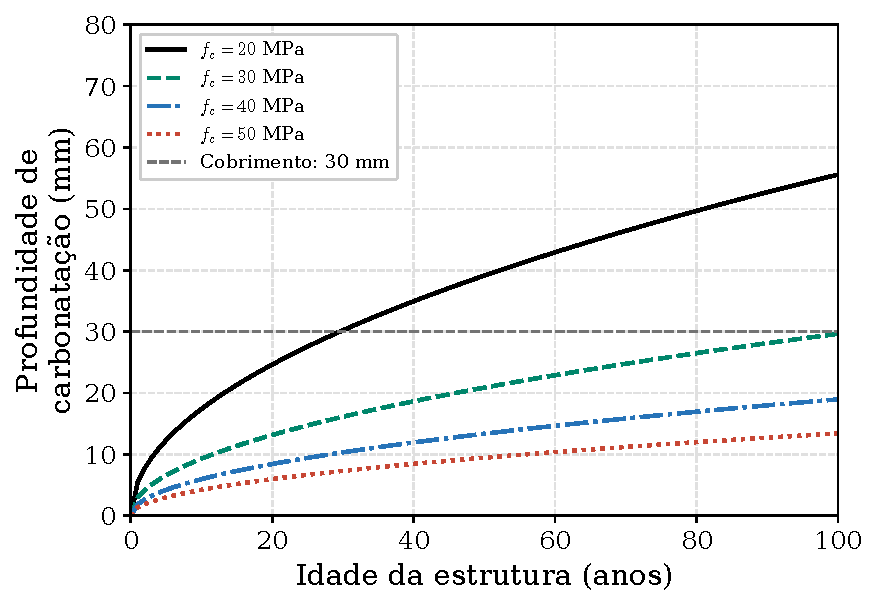
\includegraphics[width=\linewidth]{z_carbonation_fck_pt.pdf}
        \caption{Variação de $f_c$ com $UR=65\%$.}
        \label{fig:evolution_fck}
    \end{subfigure}
    \hfill
    \begin{subfigure}[b]{0.48\textwidth}
        \centering
        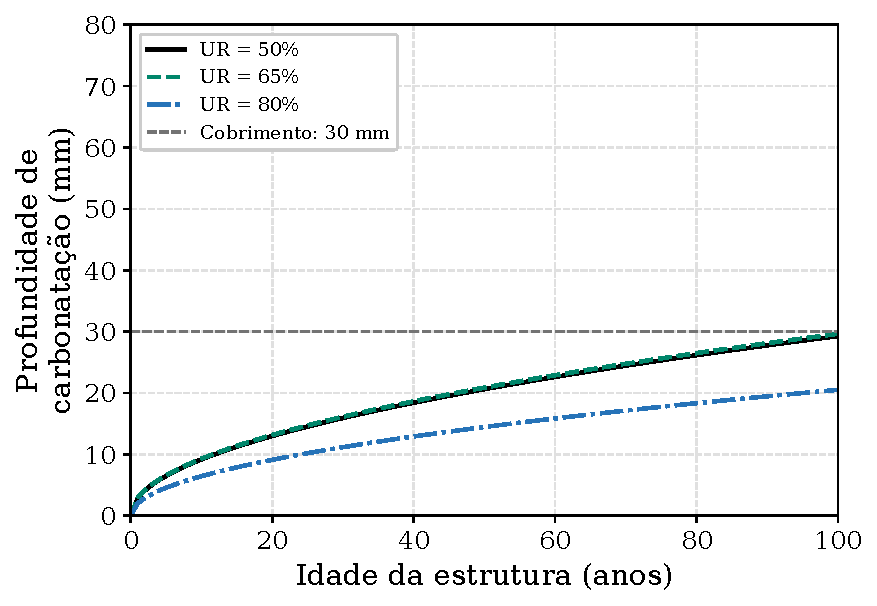
\includegraphics[width=\linewidth]{z_carbonation_rh_pt.pdf}
        \caption{Variação de $UR$ com $f_c=30$~MPa.}
        \label{fig:evolution_h}
    \end{subfigure}
    \caption{Perfis paramétricos de carbonatação para 100 anos de exposição (2000--2100), sob SSP2-4.5. O eixo horizontal representa a idade da estrutura. Perfis calculados pela Equação~\eqref{eq:y} com as hipóteses indicadas no texto.}
    \label{fig:evolucao_carb}
\end{figure}


% % =====================================================================
% % 4.2 RESISTENCIA RESIDUAL E FUNCAO DE ESTADO LIMITE  (Section_3)
% % =====================================================================
% \subsection{Resist\^encia residual \`a flex\~ao e fun\c{c}\~ao de estado limite}
% \label{subsec:resistencia_residual}

% Apresentam-se aqui os modelos para a previsão da capacidade resistente residual de vigas de concreto armado sujeitas à corrosão induzida por carbonatação. A formulação combina (i) o cálculo normativo da resistência à flexão conforme a \textcite{nbr6118} e (ii) a modelagem físico-química dos efeitos da corrosão sobre a área de aço e sobre a aderência aço--concreto, com base em \textcite{azad2010}, \textcite{val1997} e \textcite{peng2016}. Ao final, define-se a função de estado limite dependente do tempo que constitui a resposta do simulador estocástico a ser emulado.

% \subsubsection{Momento resistente da se\c{c}\~ao \'integra}
% \label{subsub:mrd0}

% O cálculo de vigas de concreto armado sem corrosão ($t \leq t_{\mathrm{ini}}$) segue as diretrizes da \textcite{nbr6118}. O momento fletor resistente de cálculo ($M_{Rd}$) é determinado pelo equilíbrio de forças na seção transversal, considerando o comportamento não linear dos materiais e o diagrama retangular simplificado de tensões no concreto comprimido. As resistências de cálculo do concreto, $f_{cd}$, e do aço, $f_{yd}$, são obtidas pela aplicação dos respectivos coeficientes de ponderação ($\gamma_c$ e $\gamma_s$), e os parâmetros geométricos do bloco de tensões ($\lambda_c$, $\alpha_c$) são definidos em função da resistência característica $f_{ck}$.

% Para seções retangulares com armadura simples, o equilíbrio entre a força normal de compressão no concreto e a força de tração na armadura escreve-se como

% \begin{equation}\label{eq:equilibrio}
% f_\alpha(\beta) = R_c(\beta) - R_s(\beta) = \sigma_{cd}\, \lambda_c\, (\beta d)\, b_w \;-\; \sigma_s(\beta)\, A_s = 0,
% \end{equation}

% \noindent em que $\beta = x/d$ é a profundidade relativa da linha neutra, $x$ é a profundidade da linha neutra, $b_w$ é a largura da seção, $d$ é a altura útil, $A_s$ é a área de armadura tracionada, $\sigma_{cd}$ é a tensão de cálculo no concreto comprimido e $\sigma_s$ é a tensão na armadura, obtida do diagrama elastoplástico definido pela norma. Devido às não linearidades física e geométrica, a raiz de $f_\alpha(\beta) = 0$ é obtida numericamente pelo método da bisseção em um intervalo predefinido. Convergido o valor de $x$, o momento resistente é calculado pela Equação~\eqref{eq:mrd_lim_resumida}:

% \begin{equation}\label{eq:mrd_lim_resumida}
% M_{Rd} = \sigma_{cd} \cdot (\lambda_c \cdot x \cdot b_w) \cdot \left(d - \tfrac{1}{2} \lambda_c x\right),
% \end{equation}

% \noindent em que o termo entre parênteses representa o braço de alavanca interno. Esse valor estabelece a linha de base de desempenho da estrutura antes do início da degradação por corrosão, denotada $M_{Rd,0}$.

% \subsubsection{Propaga\c{c}\~ao da corros\~ao e resist\^encia residual}
% \label{subsub:residual}

% Após o início da corrosão, considerado no instante $t_{\mathrm{ini}}$ definido na Seção~\ref{subsec:modelo_possan}, o modelo incorpora dois efeitos de degradação: (i) a perda de seção transversal das barras e (ii) a redução da aderência aço--concreto.

% \paragraph{Taxa de corros\~ao ajustada pela temperatura.}
% A taxa de corrosão não é considerada constante. Seguindo \textcite{peng2016}, a taxa é ajustada em função da temperatura ambiente $T(t)$ e da classe de exposição:

% \begin{equation}\label{eq:i_cor_t}
% i_{\mathrm{corr}}(T) = i_{\mathrm{corr},20} \left[ 1 + K \cdot (T - 20) \right],
% \qquad
% K =
% \begin{cases}
% 0{,}073, & T > 20\,^\circ\mathrm{C}, \\
% 0{,}025, & T < 20\,^\circ\mathrm{C}, \\
% 0, & T = 20\,^\circ\mathrm{C},
% \end{cases}
% \end{equation}

% \noindent em que $i_{\mathrm{corr},20}$ ($\mu$A/cm$^2$) é a taxa de corrosão de referência a 20\,$^\circ$C.

% \paragraph{Perda de di\^ametro e \'area efetiva.}
% Definindo o período de propagação como $t_{\mathrm{corr}} = t - t_{\mathrm{ini}}$, a redução do diâmetro original $d_{s0}$ (mm) decorre da lei de Faraday e é dada por \parencite{val1997, azad2010}:

% \begin{equation}\label{eq:d_cor}
% d_{s}(t) = d_{s0} - 0{,}0232 \cdot i_{\mathrm{corr}} \cdot t_{\mathrm{corr}},
% \end{equation}

% \noindent de modo que a área efetiva da armadura com $n_b$ barras torna-se

% \begin{equation}\label{eq:as_t}
% A_{s}(t) = n_b\, \frac{\pi\, d_{s}(t)^2}{4}.
% \end{equation}

% \paragraph{Redu\c{c}\~ao da ader\^encia.}
% A perda de aderência entre o aço corroído e o concreto é representada por um coeficiente redutor $C_f$ \parencite{azad2010}:

% \begin{equation}\label{eq:c_f}
% C_f = \min\!\left[\,1,\; \frac{5{,}0}{\, d_{s0}^{0{,}54} \left( i^{*}_{\mathrm{corr}} \cdot t_{\mathrm{corr}} \cdot 365 \right)^{0{,}19}}\right],
% \end{equation}

% \noindent em que $i^{*}_{\mathrm{corr}} = i_{\mathrm{corr}}/1000$ é expresso em A/mm$^2$ e $t_{\mathrm{corr}}$ em anos.

% \paragraph{Momento resistente degradado.}
% A resistência à flexão degradada é então calculada recompondo o equilíbrio seccional da Equação~\eqref{eq:equilibrio} com a área corroída $A_s(t)$ e aplicando o coeficiente de aderência:

% \begin{equation}\label{eq:m_res}
% M_{Rd,\mathrm{cor}}(t) = C_f \cdot M_{Rd}\!\left(A_{s}(t)\right).
% \end{equation}

% \subsubsection{Fun\c{c}\~ao de estado limite dependente do tempo}
% \label{subsec:funcao_g}

% Obtido o momento resistente degradado, avalia-se o estado limite último de flexão pela comparação entre resistência e solicitação. O momento solicitante característico total é

% \begin{equation}\label{eq:ms}
% M_S = M_{Gk} + M_{Qk},
% \end{equation}

% \noindent em que $M_{Gk}$ e $M_{Qk}$ são, respectivamente, os momentos característicos das ações permanentes e variáveis. A margem de segurança no instante $t$ --- a função de estado limite do problema --- é definida como

% \begin{equation}\label{eq:funcao_g}
% g(\mathbf{X}, t) = M_{Rd,\mathrm{cor}}(\mathbf{X}, t) - M_S(\mathbf{X}),
% \end{equation}

% \noindent em que $\mathbf{X}$ reúne todas as variáveis aleatórias do problema (propriedades de material, geometria, ambiente e ações). A interpretação física é direta:

% \begin{equation}\label{eq:dominio_falha}
% \begin{cases}
% g(\mathbf{X}, t) \geq 0, & \text{estrutura segura (estado limite não violado)}, \\[4pt]
% g(\mathbf{X}, t) < 0,  & \text{ocorrência do estado limite último}.
% \end{cases}
% \end{equation}

% O valor de $g$ indica a distância, em termos de momento fletor, entre a capacidade residual da seção corroída e a demanda estrutural. A redução progressiva de $g$ ao longo do tempo reflete a deterioração da armadura longitudinal, tanto pela perda de seção quanto pela redução da aderência. Note-se que, em razão das variáveis latentes do problema (heterogeneidade do material, flutuações ambientais, incerteza de modelo), $g(\mathbf{X}, t)$ é, para cada par $(\mathbf{x}, t)$, uma \textit{variável aleatória}, e não um valor determinístico --- precisamente a estrutura de um simulador estocástico (Seção~\ref{subsec:simulador}). Este procedimento, repetido para todos os instantes da simulação e para todas as amostras estocásticas, permitiria em princípio a determinação de curvas de confiabilidade e da probabilidade de falha por simulação direta de Monte Carlo; o custo proibitivo dessa estratégia para análises de ciclo de vida é justamente o que motiva o emulador proposto.

% \falta{a NOTA do grupo sugere um estado limite alternativo de durabilidade $g = c_{\mathrm{nom}} - y_{\mathrm{carb}}(t)$ (despassiva\c{c}\~ao: ``cobrimento menos ataque''), mais simples e diretamente lig\'avel ao Exemplo~2. Ver sugest\~ao no plano de melhorias.}

% =====================================================================
% 4.3 CONSTRUCAO DO EMULADOR DEPENDENTE DO TEMPO  (Section_4 temporal)
% =====================================================================
\subsection{Constru\c{c}\~ao do emulador dependente do tempo}
\label{subsec:construcao_emulador}

Definidos o simulador estocástico (Seção~\ref{subsec:funcao_g}) e o núcleo estatístico do emulador (Seção~\ref{sec:emuladores}), descreve-se aqui o procedimento concreto de construção do emulador PCE--GLD e sua extensão ao domínio temporal.

\subsubsection{Plano de experimentos e ajuste local}
\label{subsub:doe}

O treinamento do emulador PCE--GLD segue os passos:

\begin{enumerate}
    \item \textbf{Plano de experimentos:} um conjunto de $M$ pontos amostrais $\{\mathbf{x}^{(1)}, \dots, \mathbf{x}^{(M)}\}$ é gerado por Amostragem por Hipercubo Latino (LHS) \parencite{mckay1979}.
    \item \textbf{Avaliações estocásticas:} para cada ponto $\mathbf{x}^{(j)}$, o simulador estocástico original é executado $N$ vezes, gerando um conjunto amostral local da resposta, $\mathcal{Y}^{(j)}$.
    \item \textbf{Ajuste local da GLD:} o método dos momentos, implementado no PyGLAM com o otimizador BFGS, é utilizado para estimar os parâmetros locais ótimos $\hat{\boldsymbol{\lambda}}^{(j)}$ para cada $\mathcal{Y}^{(j)}$.
    \item \textbf{Estimação dos coeficientes da PCE:} a partir dos pares $\{\mathbf{x}^{(j)}, \hat{\boldsymbol{\lambda}}^{(j)}\}_{j=1}^M$, os coeficientes $a_{i, \boldsymbol{\alpha}}$ da Equação~\eqref{eq:pce_lambda} são calculados para cada $\lambda_i$.
\end{enumerate}

\subsubsection{Emula\c{c}\~ao dependente do tempo}
\label{subsub:temporal}

O processo de carbonatação é inerentemente dependente do tempo, exigindo que a evolução da distribuição da margem de segurança seja capturada ao longo de toda a vida em serviço da estrutura. Para tanto, o arcabouço PCE--GLD é estendido para incluir o tempo $t$ como variável de entrada contínua. Nesse esquema de emulação temporal, os parâmetros $\boldsymbol{\lambda}$ da GLD são avaliados em passos de tempo discretos, e um metamodelo de aprendizado de máquina (Seção~\ref{sec:ml}) é subsequentemente treinado para mapear o espaço conjunto de variáveis físicas $\mathbf{X}$ e tempo $t$ nos parâmetros da distribuição.

A base de treinamento do emulador temporal é construída avaliando-se o simulador estocástico em $N_t$ passos de tempo discretos $\{t_1, t_2, \dots, t_{N_t}\}$ (e.g., 0, 10, 20, 50 e 80 anos). Para cada passo $t_m$, um conjunto de $M$ amostras do vetor de entrada $\mathbf{X}^{(j)}$ é avaliado, produzindo os parâmetros locais correspondentes $\hat{\boldsymbol{\lambda}}^{(j, m)}$ via PyGLAM. A base de dados resultante $\mathcal{D}$ é definida como:

\begin{equation}
\mathcal{D} = \left\{ \left( \mathbf{x}^{(j)}, t_m \right), \hat{\boldsymbol{\lambda}}^{(j, m)} \right\} \quad \text{para } j=1,\dots,M \text{ e } m=1,\dots,N_t
\label{eq:dataset_temporal}
\end{equation}

Para prever os parâmetros da GLD em um instante arbitrário $t^*$, emprega-se o modelo de ML de múltiplas saídas descrito na Seção~\ref{subsec:redes_neurais}, que aprende o mapeamento não linear $f: (\mathbf{X}, t) \to \mathbb{R}^4$:

\begin{equation}
\hat{\boldsymbol{\lambda}}(\mathbf{X}, t) \approx \mathcal{M}_{ML}(\mathbf{X}, t; \mathbf{w}).
\label{eq:ml_temporal}
\end{equation}

Ao incluir o passo de tempo como entrada explícita, o emulador interpola os valores de $\{\lambda_1, \dots, \lambda_4\}$ entre os anos simulados, fornecendo uma evolução contínua da distribuição da margem de segurança ao longo de todo o período de análise. Duas salvaguardas são adotadas: (i) a restrição de validade $\lambda_2 > 0$ é imposta na saída do regressor (Seção~\ref{subsec:redes_neurais}); e (ii) parâmetros que exibam baixa sensibilidade às entradas podem ser excluídos do treinamento e representados por seu valor médio, decisão tomada caso a caso a partir de análise exploratória (ver Seção~\ref{subsec:exemplo1}).

\subsubsection{M\'etricas de valida\c{c}\~ao do emulador}
\label{subsec:metricas}

A similaridade estatística entre os dados de referência (\textit{ground truth}, obtidos por simulação direta) e as amostras geradas pelo emulador é avaliada por um conjunto complementar de métricas, todas aplicadas em pontos e instantes \textit{não utilizados no treinamento}:

\paragraph{Testes de ader\^encia.} O teste de Kolmogorov--Smirnov (KS) \parencite{massey1951} quantifica a máxima distância entre as funções de distribuição acumuladas empíricas, sendo sensível a discrepâncias globais; o teste de Anderson--Darling (AD) \parencite{anderson1952, scholz1987} pondera fortemente as caudas, sendo adequado para detectar desvios nas regiões extremas, justamente as mais relevantes para confiabilidade.

\paragraph{Compara\c{c}\~ao de quantis.} Erros relativos nos quantis $\{0{,}001;\, 0{,}01;\, 0{,}5;\, 0{,}99;\, 0{,}999\}$ localizam a origem de eventuais discrepâncias e quantificam diretamente a qualidade da aproximação na cauda inferior, região que governa a probabilidade de falha.

\paragraph{Diverg\^encia de Kullback--Leibler.} Para duas densidades $p(x)$ (referência) e $q(x)$ (emulador), a entropia relativa \parencite{kullback1951, cover2006}

\begin{equation}
D(p \,\|\, q) = \int p(x)\, \log \frac{p(x)}{q(x)}\, dx
\label{eq:kl_continua}
\end{equation}

\noindent é não negativa e anula-se se, e somente se, $p = q$. Embora não seja simétrica nem satisfaça a desigualdade triangular, é frequentemente útil interpretá-la como uma medida de ``distância'' entre distribuições, fornecendo um escalar global de qualidade do emulador.

% =====================================================================
% 4.4 DA DISTRIBUICAO EMULADA A RUL  (Section_5)
% =====================================================================
\subsection{Da distribui\c{c}\~ao emulada \`a vida \'util remanescente}
\label{subsec:rul}

As grandezas de interesse para a gestão de ativos --- probabilidade de falha dependente do tempo, distribuição do tempo até a despassivação, vida útil remanescente e métricas de risco --- foram definidas na Seção~\ref{subsec:rul_conceito}. Esta subseção descreve como cada uma delas é obtida a partir da distribuição condicional emulada, e não por simulação direta.

\subsubsection{Probabilidade de falha por invers\~ao da fun\c{c}\~ao quant\'ilica}
\label{subsec:pf}

Dado que o emulador fornece, para qualquer instante $t$, os parâmetros $\hat{\boldsymbol{\lambda}}(\mathbf{X},t)$ da GLD que aproxima a distribuição de $g$, a probabilidade de falha instantânea é obtida diretamente da função quantílica, sem necessidade de amostragem:

\begin{equation}
p_f(t) = \mathbb{P}\left[\, g(\mathbf{X}, t) \leq 0 \,\right] = F_{g(t)}(0) = Q^{-1}_{t}(0),
\label{eq:pf_t}
\end{equation}

\noindent em que $F_{g(t)}$ é a CDF da margem de segurança no instante $t$ e $Q_t$ a correspondente função quantílica emulada. Como a GLD é definida por sua função quantílica (Equação~\eqref{eq:GLD_quantile}) e não admite CDF em forma fechada, a inversão é realizada numericamente por bisseção em $u \in [0,1]$, procurando-se $u^{*}$ tal que $Q(u^{*};\hat{\boldsymbol{\lambda}}) = 0$; o valor $u^{*}$ é a própria probabilidade de falha. Cada avaliação custa algumas dezenas de iterações escalares, contra as milhares de execuções do simulador que a estimativa equivalente por Monte Carlo exigiria. O índice de confiabilidade generalizado associado é $\beta(t) = -\Phi^{-1}\!\left[p_f(t)\right]$, conforme a Seção~\ref{subsec:rul_conceito}.

Cabe registrar que a hipótese de monotonicidade é satisfeita de forma estrita no problema aqui tratado: a profundidade carbonatada $y(\mathbf{X},t)$ é não decrescente em $t$ --- condição imposta explicitamente pelo máximo acumulado descrito na Seção~\ref{subsec:co2} --- e o cobrimento não varia no tempo, de modo que $g$ é não crescente e uma trajetória que cruza o zero não retorna ao domínio seguro. Não há, portanto, problema de primeira passagem não monotônico, e a identidade $R(t) = 1 - p_f(t)$ vale exatamente, dispensando correções por taxa de ultrapassagem. Essa é uma vantagem do estado limite de despassivação frente a estados limites últimos com ações variáveis flutuantes, em que tal correção seria necessária.

\subsubsection{Distribui\c{c}\~ao de RUL e m\'etricas de risco}
\label{subsec:ttf_rul}

A distribuição do tempo até a despassivação, definida pela Equação~\eqref{eq:ttf}, é obtida de forma eficiente a partir do emulador. Para cada realização $\mathbf{x}$ amostrada das variáveis de projeto, a camada temporal (Seção~\ref{subsub:temporal}) fornece $\hat{\boldsymbol{\lambda}}(\mathbf{x},t)$ em qualquer instante do horizonte, do que resulta uma trajetória contínua da distribuição de $g$. O instante $T(\mathbf{x})$ é então localizado pela raiz da Equação~\eqref{eq:ttf} sobre essa trajetória, sem qualquer nova execução do modelo de carbonatação.

Fixado o instante de inspeção $t_{\mathrm{insp}}$, a amostra de tempos até a despassivação é condicionada à sobrevivência e transformada na distribuição de RUL pela Equação~\eqref{eq:rul}, da qual se extraem o valor esperado, a mediana e os quantis inferiores. As métricas de cauda VaR$_\alpha$ e CVaR$_\alpha$ (Equações~\eqref{eq:var} e \eqref{eq:cvar}) são calculadas sobre essa mesma amostra, adotando-se $\alpha = 5\%$. Todo o procedimento é pós-processamento do emulador: varrer instantes de inspeção, classes de concreto ou cenários de exposição exige apenas reavaliações da GLD interpolada.

\subsubsection{Modelagem de interven\c{c}\~oes de manuten\c{c}\~ao}
\label{subsec:manutencao}

O emulador proposto habilita a avaliação rápida de cenários de manutenção, uma vez que cada cenário exige apenas reavaliações da GLD interpolada, e não novas execuções do simulador original. Considera-se uma intervenção no instante $t_{\mathrm{man}}$ --- por exemplo, a remoção do concreto carbonatado, limpeza das armaduras e recomposição do cobrimento com argamassa de reparo realcalinizante --- cujo efeito sobre a função de estado limite é modelado por dois mecanismos \parencite{frangopol2011, vannoortwijk2009}:

\begin{enumerate}
    \item \textbf{Recuperação da margem de segurança:} o momento resistente é restaurado a uma fração $\rho \in (0, 1]$ de seu valor íntegro, $M_{Rd,\mathrm{cor}}(t_{\mathrm{man}}^{+}) = \rho \cdot M_{Rd,0}$, em que $\rho$ reflete a eficácia do reparo ($\rho = 1$ corresponde à recuperação total; valores típicos \falta{indicar faixa adotada e justificar com referência});
    \item \textbf{Reinício do relógio de iniciação:} a recomposição do cobrimento realcaliniza a vizinhança da armadura, de modo que um novo período de iniciação se desenvolve no material de reparo, $t_{\mathrm{ini}}^{\mathrm{novo}} = t_{\mathrm{man}} + \Delta t_{\mathrm{ini}}$, com $\Delta t_{\mathrm{ini}}$ governado pelo coeficiente de carbonatação do material de reparo $k_{\mathrm{rep}}$ \falta{definir distribuição de $k_{\mathrm{rep}}$; na ausência de dados, adotar $k_{\mathrm{rep}} = k$ como hipótese conservadora}.
\end{enumerate}

A trajetória resultante da margem de segurança assume o típico formato ``dente de serra'' das estruturas mantidas, e a Equação~\eqref{eq:ttf} é avaliada sobre a trajetória composta. A comparação entre as distribuições de RUL com e sem intervenção quantifica o \textit{ganho probabilístico de vida útil} proporcionado pela manutenção:

\begin{equation}
\Delta \mathrm{RUL} = \mathrm{RUL}_{\mathrm{com\;man.}}(t_{\mathrm{insp}}) - \mathrm{RUL}_{\mathrm{sem\;man.}}(t_{\mathrm{insp}}).
\label{eq:delta_rul}
\end{equation}

Adicionalmente, o emulador permite determinar de forma praticamente instantânea o \textit{instante normativo de intervenção}, definido como o primeiro tempo em que a probabilidade de falha atinge um alvo de norma,

\begin{equation}
t_{\mathrm{man}}^{*} = \inf\left\{\, t \,:\, \beta(t) \leq \beta_{\mathrm{alvo}} \,\right\},
\label{eq:t_man_otimo}
\end{equation}

\noindent adotando-se, por exemplo, $\beta_{\mathrm{alvo}} = 1{,}5$ para estados limites de serviço/durabilidade, em consonância com as recomendações do \textcite{fib2006} e do \textcite{jcss2001}. Ressalta-se que este trabalho emprega a política de limiar da Equação~\eqref{eq:t_man_otimo} como demonstração da utilidade do emulador para decisões de manutenção; a otimização completa de custo de ciclo de vida, envolvendo custos de inspeção, reparo e falha, constitui extensão natural e é apontada como trabalho futuro.
